% !TEX spellcheck = en_US



% ~~~~~~~~~~~~~~~~~~~~~~~~~~~~~~~~~~~~~~~ V
% (NC) 2026 Haluk Bingol
% github.com/halukbingol/LaTeX-Templates
%
% Licensees may copy, distribute, display, and perform the work and make derivative works 
% and remixes based on it only for non-commercial purposes. 
% ~~~~~~~~~~~~~~~~~~~~~~~~~~~~~~~~~~~~~~~ A




% =====================================================================
%  Strings in Java -- The Concepts
%  ---------------------------------------------------------------------
%  Built on hbCisLaTeXTemplate.tex with the libraries in ../../hblib/.
%  Programs and their outputs are read from codeoutput/:
%     codeoutput/<Name>.java   the program
%     codeoutput/<Name>.in     keyboard input (optional)
%     codeoutput/<Name>.txt    what it printed, made by:  sh run_examples.sh
% =====================================================================

\documentclass[aspectratio=169,10pt,compress]{beamer}

% ~~~~~~~~~~~~~~~~~~~~~~~~~~~~~~~~~~~~~~~~~~~~~~~~~~~~~~~~~~~~~ V hblib
	\usepackage{../../hblib/hblibPresentation} % lib presentation: theme, i/N, \hSection, algorithm2e, ...
	\usepackage{../../hblib/hblibCodeoutput} % lib code + output: \lstcode, \lstcodedown, ...
	\usepackage{../../hblib/hblibDatastructures} % lib data structures: \hString, \hStack, \hQueue
% ~~~~~~~~~~~~~~~~~~~~~~~~~~~~~~~~~~~~~~~~~~~~~~~~~~~~~~~~~~~~~ A hblib



\usetikzlibrary{fit}
\tikzset{
  var/.style={draw, thick, fill=blue!8, minimum width=1.1cm, minimum height=0.55cm, font=\ttfamily\small},
  obj/.style={draw, thick, rounded corners, fill=orange!10, inner sep=4pt},
  objfit/.style={draw, thick, rounded corners, orange!70!black, inner sep=0pt},
  ref/.style={-{Stealth[length=2.5mm]}, thick, blue!60!black},
  lbl/.style={font=\scriptsize\sffamily, text=gray!70!black}
}



% ~~~~~~~~~~~~~~~~~~~~~~~~~~~~~~~~~~~~~~ V doc
\title[\cisOOO-String]{
	CIS111-week09\\
	Strings
}

%\subtitle{The Concepts}

\author[Bingol]{
	Haluk O. Bingol
}

\institute[FCIS]{
    Faculty of Computer and Information Sciences\\
    Yeditepe University
}
\date{
	{\tiny \hbTimeStamp}
}

\begin{document}
% ~~~~~~~~~~~~~~~~~~~~~~~~~~~~~~~~~~~~~~ A doc




% ~~~~~~~~~~~~~~~~~~~~~~~~~~~~~~~~~~~~~~ V frm
\begin{frame}[t,fragile]
  \titlepage
\end{frame}
% ~~~~~~~~~~~~~~~~~~~~~~~~~~~~~~~~~~~~~~ A frm




% ~~~~~~~~~~~~~~~~~~~~~~~~~~~~~~~~~~~~~~ V frm
\begin{frame}[t,fragile] \frametitle{Outline}
%  \tableofcontents[hideallsubsections]
  \begin{columns}[T]
    \begin{column}{0.48\textwidth}
      \tableofcontents[sections={1-7}, hideallsubsections]
    \end{column}
    \begin{column}{0.48\textwidth}
      \tableofcontents[sections={8-14}, hideallsubsections]
    \end{column}
  \end{columns}
\end{frame}
% ~~~~~~~~~~~~~~~~~~~~~~~~~~~~~~~~~~~~~~ A frm

% ~~~~~~~~~~~~~~~~~~~~~~~~~~~~~~~~~~~~~~ V
\hSection[String]{What is String?}
% ~~~~~~~~~~~~~~~~~~~~~~~~~~~~~~~~~~~~~~ A

% ~~~~~~~~~~~~~~~~~~~~~~~~~~~~~~~~~~~~~~ V
\subsection[Text]{Text in programs}
% ~~~~~~~~~~~~~~~~~~~~~~~~~~~~~~~~~~~~~~ A




% ~~~~~~~~~~~~~~~~~~~~~~~~~~~~~~~~~~~~~~ V frm
\begin{frame}[t,fragile] \frametitle{Text is everywhere}
  \begin{columns}[T]
    \begin{column}{0.48\textwidth}
    
      Programs handle text all the time:
      \begin{itemize}\small
        
        \item names, addresses, messages
        
        \item commands typed by a user
        
        \item file and web page contents
        
        \item DNA sequences: \texttt{GATTACA}
        
        \item source code itself
      \end{itemize}
      
      \begin{block}{Definition}
        \small 
        A \hDefined{string} is a finite sequence of \textbf{characters}.
        Its \hDefined{length} is the number of characters.
      \end{block}
      
    \end{column}
    \begin{column}{0.48\textwidth}
      The string \hCode{"Hello, World"} has length 12:
      \vspace{0.6em}

      \begin{tikzpicture}
		\hString[0.42]{H,e,l,l,o,{,},\textvisiblespace,W,o,r,l,d}
      \end{tikzpicture}

      \vspace{0.6em}
      \small Each character has a \hDefined{position} (index), starting at \textbf{0}.
      The space and the comma are characters too.

      \vspace{0.4em}
      The \textbf{empty string} \hCode{""} has length 0.
    \end{column}
  \end{columns}
\end{frame}
% ~~~~~~~~~~~~~~~~~~~~~~~~~~~~~~~~~~~~~~ A frm




% ~~~~~~~~~~~~~~~~~~~~~~~~~~~~~~~~~~~~~~ V frm
\begin{frame}[t,fragile] \frametitle{A character and a string are different things}
  \small
  \begin{tabular}{@{}L{0.22\textwidth}L{0.33\textwidth}L{0.36\textwidth}@{}}
    \toprule
                       & \textbf{\hCode{char}}                  & \textbf{\hCode{String}} \\
    \midrule
    holds              & exactly \textbf{one} character           & \textbf{zero or more} characters \\
    literal            & single quotes: \hCode{'A'}              & double quotes: \hCode{"A"}, \hCode{""}, \hCode{"Ali"} \\
    kind of type       & \textbf{primitive} (a 16-bit number)     & \textbf{class} (objects, with methods) \\
    stored             & the value itself                          & a \textbf{reference} to an object \\
    default value      & \hCode{'\textbackslash u0000'}          & \hCode{null} (no object) \\
    compare with       & \texttt{==}                               & \texttt{equals(...)} \\
    \bottomrule
  \end{tabular}

  \vspace{0.8em}
	\begin{alertblock}
		{\hCode{'A'} is not \hCode{"A"}}
		\hCode{'A'} is the number 65 in disguise. 
		\hCode{"A"} is an object that \emph{contains} one character.
		Mixing them up is one of the most common beginner errors.
	\end{alertblock}
\end{frame}
% ~~~~~~~~~~~~~~~~~~~~~~~~~~~~~~~~~~~~~~ A frm

% ~~~~~~~~~~~~~~~~~~~~~~~~~~~~~~~~~~~~~~ V
%\hSection[Objects]{Strings Are Objects}{}{}
\subsection[Objects]{Strings Are Objects}{}{}
% ~~~~~~~~~~~~~~~~~~~~~~~~~~~~~~~~~~~~~~ A

% ~~~~~~~~~~~~~~~~~~~~~~~~~~~~~~~~~~~~~~ V
%\subsection[Object]{Variables hold references}
% ~~~~~~~~~~~~~~~~~~~~~~~~~~~~~~~~~~~~~~ A




% ~~~~~~~~~~~~~~~~~~~~~~~~~~~~~~~~~~~~~~ V frm
\begin{frame}[t,fragile] \frametitle{A variable holds a reference}
  \begin{columns}[T]
    \begin{column}{0.5\textwidth}

% +++++++++++++++++++++++++++++++++++++++ V lst
%: -Lst.
\begin{lstlisting}[style=codesnippet, language=Java]
String s = "Hello";
int    n = s.length();    // 5
char   c = s.charAt(1);   // 'e'
\end{lstlisting}
% +++++++++++++++++++++++++++++++++++++++ A lst



	\begin{itemize}\small
	
		\item 
		\hCode{s} does not contain the letters; 
		it \textbf{refers} (points) to a \hCode{String} object
		
		\item 
		We \textbf{ask the object}: \hCode{s.length()}, \hCode{s.charAt(1)}

		\item 
		The object knows its characters and offers about 70 methods
		
	\end{itemize}
    \end{column}
    \begin{column}{0.46\textwidth}

      \begin{center}
      \begin{tikzpicture}
        \node[var] (s) at (0,0) {s};
        \node[lbl, above=1pt of s] {variable};
\begin{scope}[shift={(2.2,-0.200)}]\hString[0.4]{H,e,l,l,o}\end{scope}
\node[objfit, fit={(2.080,-0.320) (4.320,0.500)}] (o) {};

        \node[lbl, above=1pt of o] {String object};
        \draw[ref] (s) -- (o);
        \node[var] (n) at (0,-1.4) {5};
        \node[lbl, left=2pt of n] {\texttt{n}};
        \node[var] (c) at (0,-2.3) {'e'};
        \node[lbl, left=2pt of c] {\texttt{c}};
        \node[lbl, align=left, anchor=west] at (1.2,-1.85) {primitives:\\the value itself};
      \end{tikzpicture}
      \end{center}
      
    \end{column}
  \end{columns}
\end{frame}
% ~~~~~~~~~~~~~~~~~~~~~~~~~~~~~~~~~~~~~~ A frm





% ~~~~~~~~~~~~~~~~~~~~~~~~~~~~~~~~~~~~~~ V frm
\begin{frame}[t,fragile] \frametitle{Nothing, empty, or blank?}
  \begin{columns}[T]
    \begin{column}{0.5\textwidth}
    
      \begin{center}
      \begin{tikzpicture}
        \node[var] (a) at (0,0) {a};
        \node[lbl, above=1pt of a] {variable};

        \node[font=\ttfamily\small, anchor=west] at (1.0,0) {null \quad (no object)};
        \node[var] (b) at (0,-1.3) {b};
\node[objfit, minimum width=0.5cm, minimum height=0.5cm] (ob) at (1.65,-1.3) {};

        \node[lbl, right=2pt of ob] {length 0};
        \draw[ref] (b) -- (ob);
        \node[var] (c) at (0,-2.6) {c};
\begin{scope}[shift={(1.4,-2.800)}]\hString[0.4]{\textvisiblespace,\textvisiblespace,\textvisiblespace}\end{scope}
\node[objfit, fit={(1.280,-2.920) (2.720,-2.100)}] (oc) {};

        \node[lbl, right=2pt of oc] {length 3};
        \draw[ref] (c) -- (oc);
      \end{tikzpicture}
      \end{center}


% +++++++++++++++++++++++++++++++++++++++ V lst
%: -Lst.
\begin{lstlisting}[style=codesnippet, language=Java]
String a = null;
String b = "";
String c = "   ";
\end{lstlisting}
% +++++++++++++++++++++++++++++++++++++++ A lst



    \end{column}
    \begin{column}{0.46\textwidth}
      \small
      \begin{tabular}{@{}lccc@{}}
        \toprule
                               & \texttt{a}     & \texttt{b}    & \texttt{c} \\
        \midrule
        \hCode{x == null}     & true           & false         & false \\
        \hCode{x.isEmpty()}   & \emph{error}   & true          & false \\
        \hCode{x.isBlank()}   & \emph{error}   & true          & true \\
        \bottomrule
      \end{tabular}

      \vspace{0.6em}
      
	\begin{alertblock}{NullPointerException}
		\small Calling a method on \hCode{null} fails: there is no object to ask.
		Check \hCode{x != null} first, or write \hCode{"text".equals(x)}.
	\end{alertblock}
	
    \end{column}
  \end{columns}
\end{frame}
% ~~~~~~~~~~~~~~~~~~~~~~~~~~~~~~~~~~~~~~ A frm

% ~~~~~~~~~~~~~~~~~~~~~~~~~~~~~~~~~~~~~~ V
\subsection[Index]{Positions and pieces}
% ~~~~~~~~~~~~~~~~~~~~~~~~~~~~~~~~~~~~~~ A




% ~~~~~~~~~~~~~~~~~~~~~~~~~~~~~~~~~~~~~~ V frm
\begin{frame}[t,fragile] \frametitle{Positions start at 0}
  \begin{center}
    \begin{tikzpicture}\hString[0.55]{Y,e,d,i,t,e,p,e}[4][8]\end{tikzpicture}
  \end{center}
  \vspace{0.3em}
  \small
  \begin{tabular}{@{}L{0.34\textwidth}L{0.18\textwidth}L{0.4\textwidth}@{}}
    \toprule
    \textbf{Expression}            & \textbf{Value}       & \textbf{Why} \\
    \midrule
    \hCode{s.length()}            & \hCode{8}           & 8 characters \\
    \hCode{s.charAt(0)}           & \hCode{'Y'}         & first index is 0 \\
    \hCode{s.charAt(s.length()-1)}& \hCode{'e'}         & last index is \hCode{length-1} \\
    \hCode{s.substring(4, 8)}     & \hCode{"tepe"}      & from 4 \textbf{up to, not including}, 8 (highlighted) \\
    \hCode{s.indexOf("tepe")}     & \hCode{4}           & where it starts; \hCode{-1} if not found \\
    \hCode{s.charAt(8)}           & \emph{exception}     & index 8 does not exist \\
    \bottomrule
  \end{tabular}

  \vspace{0.4em}
  \hRemark{Rule of thumb:} \hCode{substring(b, e)} has length \hCode{e - b}.
\end{frame}
% ~~~~~~~~~~~~~~~~~~~~~~~~~~~~~~~~~~~~~~ A frm




% ~~~~~~~~~~~~~~~~~~~~~~~~~~~~~~~~~~~~~~
%\subsection{null}

% ~~~~~~~~~~~~~~~~~~~~~~~~~~~~~~~~~~~~~~ V
%\hSection[Immutable]{Immutability}{}{}
% ~~~~~~~~~~~~~~~~~~~~~~~~~~~~~~~~~~~~~~ A

% ~~~~~~~~~~~~~~~~~~~~~~~~~~~~~~~~~~~~~~ V
\subsection[Immutable]{A String never changes}
% ~~~~~~~~~~~~~~~~~~~~~~~~~~~~~~~~~~~~~~ A




% ~~~~~~~~~~~~~~~~~~~~~~~~~~~~~~~~~~~~~~ V frm
\begin{frame}[t,fragile] \frametitle{A String never changes}
  \begin{columns}[T]
    \begin{column}{0.44\textwidth}


% +++++++++++++++++++++++++++++++++++++++ V lst
%: -Lst.
\begin{lstlisting}[style=codesnippet, language=Java]
String s = "java";
s.toUpperCase();      // result lost!
s = s.toUpperCase();  // s now refers
                      // to a new object
\end{lstlisting}
% +++++++++++++++++++++++++++++++++++++++ A lst



	\begin{itemize}\small
		\item 
		Every ``changing'' method (
		\hCode{toUpperCase}, 
		\hCode{replace}, 
		\hCode{trim}, \dots)
              \textbf{returns a new} \hCode{String}

		\item The original object is never modified

		\item An object nobody refers to is removed by the \textbf{garbage collector}
	\end{itemize}
	
    \end{column}
    \begin{column}{0.52\textwidth}
    
      \begin{center}
      \begin{tikzpicture}
        \node[lbl] at (2,1.2) {\normalsize \hCode{s = s.toUpperCase();}};
        
        \node[lbl] at (0,0.9) {before};
        \node[var] (s1) at (0,0) {s};
        
	\begin{scope}[shift={(1.6,-0.200)}]\hString[0.4]{j,a,v,a}\end{scope}
	\node[objfit, fit={(1.480,-0.320) (3.320,0.500)}] (o1) {};

        \draw[ref] (s1) -- (o1);

        \node[lbl] at (0,-1.3) {after};
        \node[var] (s2) at (0,-2.0) {s};
        
        \begin{scope}[opacity=0.4]
		\begin{scope}[shift={(1.6,-1.800)}]\hString[0.4]{j,a,v,a}\end{scope}
		\node[objfit, fit={(1.480,-1.920) (3.320,-1.100)}] (o2) {};
	\end{scope}
        
	\begin{scope}[shift={(1.6,-3.000)}]\hString[0.4]{J,A,V,A}[0][4]\end{scope}
	\node[objfit, fit={(1.480,-3.120) (3.320,-2.300)}] (o3) {};

        \draw[ref] (s2) -- (o3.west);
        
        \node[lbl, right=2pt of o2, align=left] {unchanged,\\garbage now};
        \node[lbl, right=2pt of o3] {new object};
      \end{tikzpicture}
      \end{center}
      
    \end{column}
  \end{columns}
\end{frame}
% ~~~~~~~~~~~~~~~~~~~~~~~~~~~~~~~~~~~~~~ A frm




% ~~~~~~~~~~~~~~~~~~~~~~~~~~~~~~~~~~~~~~ V frm
\begin{frame}[t,fragile] \frametitle{Why are strings immutable?}
  \begin{columns}[T]
    \begin{column}{0.48\textwidth}
      \begin{block}{Safe sharing}
        \small Many variables can refer to the same string. Nobody can change it under the others' feet.
      \end{block}
      \begin{block}{Security}
        \small A file name or URL checked once cannot be altered after the check.
      \end{block}
      \begin{block}{Threads}
        \small Immutable objects can be used by many threads without locks.
      \end{block}
    \end{column}
    \begin{column}{0.48\textwidth}
      \begin{block}{Hashing}
        \small Strings are the most common \texttt{HashMap} keys. Their hash code never changes,
        so it is computed once and cached.
      \end{block}
      \begin{block}{The string pool}
        \small Equal literals can share one object, saving memory (next section).
      \end{block}
      \begin{alertblock}{The price}
        \small Building a long string piece by piece creates many temporary objects.
        That is what \texttt{StringBuilder} is for.
      \end{alertblock}
    \end{column}
  \end{columns}
\end{frame}
% ~~~~~~~~~~~~~~~~~~~~~~~~~~~~~~~~~~~~~~ A frm

% ~~~~~~~~~~~~~~~~~~~~~~~~~~~~~~~~~~~~~~ V
\subsection[Builder]{Building strings}
% ~~~~~~~~~~~~~~~~~~~~~~~~~~~~~~~~~~~~~~ A




% ~~~~~~~~~~~~~~~~~~~~~~~~~~~~~~~~~~~~~~ V frm
\begin{frame}[t,fragile] \frametitle{Building a string: \texttt{+} versus \texttt{StringBuilder}}
  \begin{columns}[T]
    \begin{column}{0.48\textwidth}


% +++++++++++++++++++++++++++++++++++++++ V lst
%: -Lst.
\begin{lstlisting}[style=codesnippet, language=Java]
String s = "";
for (int i = 0; i < n; i++){
    s = s + "x";    // new object each time
}
\end{lstlisting}
% +++++++++++++++++++++++++++++++++++++++ A lst



      \small Step $k$ copies the $k$ characters built so far into a new object. In total:
      \[
      	1 + 2 + \dots + n = \frac{n(n+1)}{2} \in O(n^{2})
      \]
      \small For $n = 100\,000$ that is about 5 billion copied characters.
    \end{column}
    \begin{column}{0.48\textwidth}


% +++++++++++++++++++++++++++++++++++++++ V lst
%: -Lst.
\begin{lstlisting}[style=codesnippet, language=Java]
StringBuilder sb = new StringBuilder();
for (int i = 0; i < n; i++){
    sb.append("x"); // same buffer
}
String s = sb.toString();
\end{lstlisting}
% +++++++++++++++++++++++++++++++++++++++ A lst



      \small A \texttt{StringBuilder} is a \textbf{mutable} buffer with spare room (capacity).
      When full, it doubles; the total copying stays $O(n)$.
      \begin{center}
      
\begin{tikzpicture}
        \hString[0.35]{x,x,x,x,x,\ ,\ ,\ }[5][8]
        \node[lbl, anchor=west] at (2.9,0.17) {spare capacity};
      \end{tikzpicture}
      \end{center}
    \end{column}
  \end{columns}
\end{frame}
% ~~~~~~~~~~~~~~~~~~~~~~~~~~~~~~~~~~~~~~ A frm

% ~~~~~~~~~~~~~~~~~~~~~~~~~~~~~~~~~~~~~~ V
%\hSection[Equality]{Equality and Order}{}{}
\hSection[Comparison]{Comparing Strings}
% ~~~~~~~~~~~~~~~~~~~~~~~~~~~~~~~~~~~~~~ A

% ~~~~~~~~~~~~~~~~~~~~~~~~~~~~~~~~~~~~~~ V
\subsection[Same]{Same object or same text?}
% ~~~~~~~~~~~~~~~~~~~~~~~~~~~~~~~~~~~~~~ A




% ~~~~~~~~~~~~~~~~~~~~~~~~~~~~~~~~~~~~~~ V frm
\begin{frame}[t,fragile] \frametitle{Same object or same text?}
  \begin{columns}[T]
    \begin{column}{0.46\textwidth}


% +++++++++++++++++++++++++++++++++++++++ V lst
%: -Lst.
\begin{lstlisting}[style=codesnippet, language=Java]
String a = new String("ali");
String b = new String("ali");
String c = a;

a == b        // false
a.equals(b)   // true
a == c        // true
\end{lstlisting}
% +++++++++++++++++++++++++++++++++++++++ A lst


      \begin{itemize}\small
        \item \hCode{==} compares \textbf{references}: is it the \emph{same object}?
        \item \hCode{equals} compares \textbf{characters}: is it the \emph{same text}?
      \end{itemize}
    \end{column}
    \begin{column}{0.5\textwidth}
    
      \begin{center}
      \begin{tikzpicture}
        \node[var] (a) at (0,0) {a};
        \node[var] (c) at (0,-0.9) {c};
        \node[var] (b) at (0,-2.3) {b};
\begin{scope}[shift={(2.2,-0.650)}]\hString[0.4]{a,l,i}\end{scope}
\node[objfit, fit={(2.080,-0.770) (3.520,0.050)}] (o1) {};
\begin{scope}[shift={(2.2,-2.500)}]\hString[0.4]{a,l,i}\end{scope}
\node[objfit, fit={(2.080,-2.620) (3.520,-1.800)}] (o2) {};

        \draw[ref] (a) -- (o1);
        \draw[ref] (c) -- (o1);
        \draw[ref] (b) -- (o2);
      \end{tikzpicture}
      \end{center}
      
      \begin{alertblock}{Rule}
        \small Compare strings with \hCode{equals} (or \hCode{equalsIgnoreCase}), 
        never with \hCode{==}.
      \end{alertblock}
    \end{column}
  \end{columns}
\end{frame}
% ~~~~~~~~~~~~~~~~~~~~~~~~~~~~~~~~~~~~~~ A frm




% ~~~~~~~~~~~~~~~~~~~~~~~~~~~~~~~~~~~~~~ V frm
\begin{frame}[t,fragile] \frametitle{The string pool}
  \begin{columns}[T]
    \begin{column}{0.46\textwidth}


% +++++++++++++++++++++++++++++++++++++++ V lst
%: -Lst.
\begin{lstlisting}[style=codesnippet, language=Java]
String x = "java";             // pool
String y = "java";             // same
String z = new String("java"); // new

x == y            // true
x == z            // false
x == z.intern()   // true
\end{lstlisting}
% +++++++++++++++++++++++++++++++++++++++ A lst



      \small \textbf{Literals} are kept in a \textbf{pool}: equal literals share one object.
      \hCode{new} always makes a new object. 
      \hCode{intern()} returns the pooled copy.
      
    \end{column}
    \begin{column}{0.5\textwidth}
    
      \begin{center}
      \begin{tikzpicture}
        \node[var] (x) at (0,0.2) {x};
        \node[var] (y) at (0,-0.7) {y};
        \node[var] (z) at (0,-2.4) {z};
\begin{scope}[shift={(2.2,-0.450)}]\hString[0.4]{j,a,v,a}\end{scope}
\node[objfit, fit={(2.080,-0.570) (3.920,0.250)}] (p) {};

        \node[draw, dashed, rounded corners, fit=(p), inner sep=8pt, label={[lbl]above:string pool}] {};
\begin{scope}[shift={(2.2,-2.600)}]\hString[0.4]{j,a,v,a}\end{scope}
\node[objfit, fit={(2.080,-2.720) (3.920,-1.900)}] (h) {};

        \node[lbl, below=2pt of h] {ordinary heap object};
        \draw[ref] (x) -- (p);
        \draw[ref] (y) -- (p);
        \draw[ref] (z) -- (h);
      \end{tikzpicture}
      \end{center}
      
      \small \hRemark{Why it still matters:} 
      \hCode{x == y} being \hCode{true} for literals
      makes \hCode{==} \emph{look} correct in small tests, 
      then fail on user input.
    \end{column}
  \end{columns}
\end{frame}
% ~~~~~~~~~~~~~~~~~~~~~~~~~~~~~~~~~~~~~~ A frm




% ~~~~~~~~~~~~~~~~~~~~~~~~~~~~~~~~~~~~~~ V
%\hSection[Compare]{Comparing Strings}{}{}
% ~~~~~~~~~~~~~~~~~~~~~~~~~~~~~~~~~~~~~~ A


% ~~~~~~~~~~~~~~~~~~~~~~~~~~~~~~~~~~~~~~ V
\subsection[Bug]{equals, not ==}
% ~~~~~~~~~~~~~~~~~~~~~~~~~~~~~~~~~~~~~~ A




% ~~~~~~~~~~~~~~~~~~~~~~~~~~~~~~~~~~~~~~ V frm
\begin{frame}[t,fragile] \frametitle{The most famous string bug}
  \lstcoderightstep[0.7][basicstyle=\ttfamily\scriptsize][basicstyle=\ttfamily\scriptsize]{codeoutput/EqualsTrap.java}{Java}{codeoutput/EqualsTrap.txt}

  \vspace{0.3em}
  \small The user typed \texttt{yes}, yet \hCode{answer == "yes"} is \hCode{false}: \hCode{==} asks whether they are
  the \textbf{same object}. 
  \hRemark{Always compare text with} \hCode{equals}: \hCode{answer.equals("yes")}.
\end{frame}
% ~~~~~~~~~~~~~~~~~~~~~~~~~~~~~~~~~~~~~~ A frm


% ~~~~~~~~~~~~~~~~~~~~~~~~~~~~~~~~~~~~~~ V
\subsection[Rules]{Comparing rules}
% ~~~~~~~~~~~~~~~~~~~~~~~~~~~~~~~~~~~~~~ A




% ~~~~~~~~~~~~~~~~~~~~~~~~~~~~~~~~~~~~~~ V frm
\begin{frame}[t,fragile] \frametitle{Comparing strings: the rules}
  \small
  \begin{tabular}{@{}L{0.4\textwidth}L{0.5\textwidth}@{}}
    \toprule
    \textbf{Question}                     & \textbf{Write} \\
    \midrule
    same text?                            & \hCode{a.equals(b)} \\
    same text, ignoring case?             & \hCode{a.equalsIgnoreCase(b)} \\
    which comes first?                    & \hCode{a.compareTo(b) < 0} \\
    is it empty?                          & \hCode{a.isEmpty()} \\
    does it contain \texttt{"x"}?         & \hCode{a.contains("x")} \\
    does it start with \texttt{"Dr."}?    & \hCode{a.startsWith("Dr.")} \\
    \bottomrule
  \end{tabular}

  \vspace{0.8em}
  \begin{alertblock}{Never}
    \hCode{if (a == b)} with strings. 
    It may even work in a small test (with literals), then fail with user input.
  \end{alertblock}
\end{frame}
% ~~~~~~~~~~~~~~~~~~~~~~~~~~~~~~~~~~~~~~ A frm


% ~~~~~~~~~~~~~~~~~~~~~~~~~~~~~~~~~~~~~~ V
\subsection[Order]{Dictionary order}
% ~~~~~~~~~~~~~~~~~~~~~~~~~~~~~~~~~~~~~~ A




% ~~~~~~~~~~~~~~~~~~~~~~~~~~~~~~~~~~~~~~ V frm
\begin{frame}[t,fragile] \frametitle{Dictionary order: \texttt{compareTo}}

	\vspace{-0.2cm}
	
	\small 
	\[
		\hCode{a.compareTo(b)} =
		\begin{cases}
			\textbf{negative} & \text{ \hCode{a} comes first}, \\
			\textbf{0} & \text{equal},\\
			\textbf{positive} & \text{\hCode{a} comes after}.
		\end{cases}
	\]  

	It compares character codes from left to right.

	\vspace{0.4em}
	\begin{tabular}{@{}L{0.32\textwidth}L{0.08\textwidth}L{0.5\textwidth}@{}}
		\toprule
		\textbf{Call}                                  & \textbf{Result} & \textbf{Reason} \\
		\midrule
		\hCode{"apple".compareTo("banana")}           & $-1$  & \hCode{'a'} (97) $-$ \hCode{'b'} (98) \\
		\hCode{"Apple".compareTo("apple")}            & $-32$ & \hCode{'A'} (65) $-$ \hCode{'a'} (97): capitals first \\
		\hCode{"Zebra".compareTo("apple")}            & $-7$  & \hCode{'Z'} (90) $<$ \hCode{'a'} (97) \\
		\hCode{"app".compareTo("apple")}              & $-2$  & a prefix comes first: $3 - 5$ \\
		\hCode{"çay".compareTo("zeytin")}             & $109$ & \hCode{'ç'} (231) $>$ \hCode{'z'} (122) \\
		\bottomrule
	\end{tabular}

	\vspace{0.6em}
	\begin{alertblock}{Character-code order is not the alphabet}
		\small Upper case before lower case, and 
		Turkish letters (ç, ğ, ı, ö, ş, ü) after \texttt{z}.
		For real alphabetical order use 
		\hCode{compareToIgnoreCase} or a 
		\hCode{Collator} for the language.
	\end{alertblock}
\end{frame}
% ~~~~~~~~~~~~~~~~~~~~~~~~~~~~~~~~~~~~~~ A frm



% ~~~~~~~~~~~~~~~~~~~~~~~~~~~~~~~~~~~~~~ V
\hSection[Plus]{\hCode{+} operator}
% ~~~~~~~~~~~~~~~~~~~~~~~~~~~~~~~~~~~~~~ A




% ~~~~~~~~~~~~~~~~~~~~~~~~~~~~~~~~~~~~~~ V
\subsection[Plus]{Joining with +}
% ~~~~~~~~~~~~~~~~~~~~~~~~~~~~~~~~~~~~~~ A




% ~~~~~~~~~~~~~~~~~~~~~~~~~~~~~~~~~~~~~~ V frm
\begin{frame}[t,fragile] \frametitle{Joining strings with \texttt{+}}
	\lstcoderightstep[0.75]
		[basicstyle=\ttfamily\scriptsize]
		[basicstyle=\ttfamily\scriptsize]
			{codeoutput/Greeting.java}{Java}
			{codeoutput/Greeting.txt}

	\vspace{0.3em}
	\small \hRemark{Look at the last line:} 
	\hCode{"Class of " + year} is a string, 
	then \hCode{+ 4} appends ``4''.
	Use parentheses to add numbers first.
\end{frame}
% ~~~~~~~~~~~~~~~~~~~~~~~~~~~~~~~~~~~~~~ A frm




% ~~~~~~~~~~~~~~~~~~~~~~~~~~~~~~~~~~~~~~ V frm
\begin{frame}[t,fragile] \frametitle{Puzzle: what does \texttt{+} do here?}
	\lstcoderightstep[0.7]
		[basicstyle=\ttfamily\scriptsize]
		[basicstyle=\ttfamily\scriptsize]
			{codeoutput/PlusPuzzle.java}{Java}
			{codeoutput/PlusPuzzle.txt}

	\vspace{0.3em}
	\small \hCode{+} works \textbf{left to right}. 
	Number $+$ number adds; 
	as soon as one side is a \hCode{String}, it joins.
	Two \hCode{char}s are numbers: \hCode{'a' + 'b'} is $97 + 98 = 195$.
\end{frame}
% ~~~~~~~~~~~~~~~~~~~~~~~~~~~~~~~~~~~~~~ A frm




% ~~~~~~~~~~~~~~~~~~~~~~~~~~~~~~~~~~~~~~ V
\hSection[API]{\hCode{String} API}{}{}
% ~~~~~~~~~~~~~~~~~~~~~~~~~~~~~~~~~~~~~~ A




% ~~~~~~~~~~~~~~~~~~~~~~~~~~~~~~~~~~~~~~ V
%\hSection[Examples]{Examples}{}{}
% ~~~~~~~~~~~~~~~~~~~~~~~~~~~~~~~~~~~~~~ A

% ~~~~~~~~~~~~~~~~~~~~~~~~~~~~~~~~~~~~~~ V
\subsection[Create]{Creating strings}
% ~~~~~~~~~~~~~~~~~~~~~~~~~~~~~~~~~~~~~~ A




% ~~~~~~~~~~~~~~~~~~~~~~~~~~~~~~~~~~~~~~ V frm
\begin{frame}[t,fragile] \frametitle{Five ways to get a String}
	\lstcoderightstep[0.7]
		[basicstyle=\ttfamily\scriptsize]
		[basicstyle=\ttfamily\tiny]
			{codeoutput/Create.java}{Java}
			{codeoutput/Create.txt}
\end{frame}
% ~~~~~~~~~~~~~~~~~~~~~~~~~~~~~~~~~~~~~~ A frm



% ~~~~~~~~~~~~~~~~~~~~~~~~~~~~~~~~~~~~~~ V
\subsection[Length]{Length and characters}
% ~~~~~~~~~~~~~~~~~~~~~~~~~~~~~~~~~~~~~~ A




% ~~~~~~~~~~~~~~~~~~~~~~~~~~~~~~~~~~~~~~ V frm
\begin{frame}[t,fragile] \frametitle{\texttt{length()} and \texttt{charAt(i)}}
	\lstcoderightstep[0.7]
		[basicstyle=\ttfamily\scriptsize]
		[basicstyle=\ttfamily\tiny]
			{codeoutput/LengthCharAt.java}{Java}
			{codeoutput/LengthCharAt.txt}

	\vspace{0.3em}
	\small Valid indices are \hCode{0} to \hCode{length()-1}. 
	A \hCode{char} is a number: \hCode{(int) c} shows its code.
\end{frame}
% ~~~~~~~~~~~~~~~~~~~~~~~~~~~~~~~~~~~~~~ A frm




% ~~~~~~~~~~~~~~~~~~~~~~~~~~~~~~~~~~~~~~ V
\subsection[Substring]{Pieces of a string}
% ~~~~~~~~~~~~~~~~~~~~~~~~~~~~~~~~~~~~~~ A




% ~~~~~~~~~~~~~~~~~~~~~~~~~~~~~~~~~~~~~~ V frm
\begin{frame}[t,fragile] \frametitle{\texttt{substring(begin, end)}}
\begin{columns}[T]
	\begin{column}{0.66\textwidth}
		\lstcode
			[basicstyle=\ttfamily\scriptsize]{codeoutput/Substring.java}{Java}
	\end{column}
	\begin{column}{0.32\textwidth}
		\begin{center}
		\begin{tikzpicture}
			\hString[0.32]{H,e,l,l,o,{,},\textvisiblespace,W,o,r,l,d}[7][12]
		\end{tikzpicture}
		\end{center}
		\small \hCode{substring(7, 12)}: from index 7 \textbf{up to, not including} 12.
		\vspace{0.3em}

		\uncover<2->{
			\lstoutput
				[basicstyle=\ttfamily\scriptsize]{codeoutput/Substring.txt}
		}
	\end{column}
\end{columns}
\end{frame}
% ~~~~~~~~~~~~~~~~~~~~~~~~~~~~~~~~~~~~~~ A frm



% ~~~~~~~~~~~~~~~~~~~~~~~~~~~~~~~~~~~~~~ V
\subsection[Search]{Searching}
% ~~~~~~~~~~~~~~~~~~~~~~~~~~~~~~~~~~~~~~ A




% ~~~~~~~~~~~~~~~~~~~~~~~~~~~~~~~~~~~~~~ V frm
\begin{frame}[t,fragile] \frametitle{Searching: \texttt{indexOf}, \texttt{contains}, \dots}
	\vspace{-0.2cm}
	\lstcoderightstep[0.75]
		[basicstyle=\ttfamily\scriptsize]
		[basicstyle=\ttfamily\scriptsize]
			{codeoutput/Search.java}{Java}
			{codeoutput/Search.txt}

	\vspace{0.3em}
	\small 
	\hCode{indexOf} returns \hCode{-1} when not found. 
	The loop finds every occurrence by starting after the previous one.
\end{frame}
% ~~~~~~~~~~~~~~~~~~~~~~~~~~~~~~~~~~~~~~ A frm




% ~~~~~~~~~~~~~~~~~~~~~~~~~~~~~~~~~~~~~~ V
\subsection[Compare]{Comparing}
% ~~~~~~~~~~~~~~~~~~~~~~~~~~~~~~~~~~~~~~ A




% ~~~~~~~~~~~~~~~~~~~~~~~~~~~~~~~~~~~~~~ V frm
\begin{frame}[t,fragile] \frametitle{Comparing: \texttt{equals} and \texttt{compareTo}}
	\lstcoderightstep[0.75]
		[basicstyle=\ttfamily\scriptsize]
		[basicstyle=\ttfamily\scriptsize]
			{codeoutput/Compare.java}{Java}
			{codeoutput/Compare.txt}

	\vspace{0.3em}
	\small 
	\hCode{==} asks ``same object?''; 
	\hCode{equals} asks ``same text?''. 
	\hCode{compareTo} is negative, zero or positive.
\end{frame}
% ~~~~~~~~~~~~~~~~~~~~~~~~~~~~~~~~~~~~~~ A frm




% ~~~~~~~~~~~~~~~~~~~~~~~~~~~~~~~~~~~~~~ V
\subsection[Case]{Upper and lower case}
% ~~~~~~~~~~~~~~~~~~~~~~~~~~~~~~~~~~~~~~ A




% ~~~~~~~~~~~~~~~~~~~~~~~~~~~~~~~~~~~~~~ V frm
\begin{frame}[t,fragile] \frametitle{Upper and lower case: the Turkish \texttt{i}}
  \lstcoderightstep[0.7][basicstyle=\ttfamily\scriptsize][basicstyle=\ttfamily\scriptsize]{codeoutput/Case.java}{Java}{codeoutput/Case.txt}

  \vspace{0.3em}
  \small \hRemark{Pitfall:} 
  \hCode{toUpperCase()} without a locale uses the computer's language. 
  On a Turkish
  computer \hCode{"title".toUpperCase()} is \hCode{"TİTLE"}. 
  Use \hCode{Locale.ROOT} for program text (keywords, file names).
\end{frame}
% ~~~~~~~~~~~~~~~~~~~~~~~~~~~~~~~~~~~~~~ A frm




% ~~~~~~~~~~~~~~~~~~~~~~~~~~~~~~~~~~~~~~ V
\subsection[Transform]{Trimming, splitting, joining}
% ~~~~~~~~~~~~~~~~~~~~~~~~~~~~~~~~~~~~~~ A




% ~~~~~~~~~~~~~~~~~~~~~~~~~~~~~~~~~~~~~~ V frm
\begin{frame}[t,fragile] \frametitle{Trimming, splitting and joining}
  \lstcoderightstep[0.7][basicstyle=\ttfamily\scriptsize][basicstyle=\ttfamily\tiny]{codeoutput/TrimSplit.java}{Java}{codeoutput/TrimSplit.txt}

  \vspace{0.3em}
  \small \texttt{split} takes a \textbf{regular expression}: 
  \hCode{"\textbackslash\textbackslash s+"} means 
  ``one or more white-space characters''.
\end{frame}
% ~~~~~~~~~~~~~~~~~~~~~~~~~~~~~~~~~~~~~~ A frm




% ~~~~~~~~~~~~~~~~~~~~~~~~~~~~~~~~~~~~~~ V
\subsection[Replace]{Replacing}
% ~~~~~~~~~~~~~~~~~~~~~~~~~~~~~~~~~~~~~~ A




% ~~~~~~~~~~~~~~~~~~~~~~~~~~~~~~~~~~~~~~ V frm
\begin{frame}[t,fragile] \frametitle{Replacing and repeating}
  \lstcoderightstep[0.7][basicstyle=\ttfamily\scriptsize][basicstyle=\ttfamily\scriptsize]{codeoutput/Replace.java}{Java}{codeoutput/Replace.txt}

  \vspace{0.3em}
  \small The last line proves it again: 
  none of these methods changes \hCode{s}; 
  each returns a new string.
\end{frame}
% ~~~~~~~~~~~~~~~~~~~~~~~~~~~~~~~~~~~~~~ A frm




% ~~~~~~~~~~~~~~~~~~~~~~~~~~~~~~~~~~~~~~ V
\subsection[Format]{Formatting}
% ~~~~~~~~~~~~~~~~~~~~~~~~~~~~~~~~~~~~~~ A




% ~~~~~~~~~~~~~~~~~~~~~~~~~~~~~~~~~~~~~~ V frm
\begin{frame}[t,fragile] \frametitle{Formatting numbers and text}
  \lstcoderightstep[0.7][basicstyle=\ttfamily\scriptsize][basicstyle=\ttfamily\scriptsize]{codeoutput/Format.java}{Java}{codeoutput/Format.txt}

  \vspace{0.3em}
  \small 
  \hCode{\%s} text, 
  \hCode{\%d} integer, 
  \hCode{\%.2f} two decimals, 
  \hCode{\%-8s} left-aligned in 8 columns, 
  \hCode{\%n} new line.
  With the Turkish locale the decimal separator is a comma.
\end{frame}
% ~~~~~~~~~~~~~~~~~~~~~~~~~~~~~~~~~~~~~~ A frm




% ~~~~~~~~~~~~~~~~~~~~~~~~~~~~~~~~~~~~~~ V
\subsection[Convert]{Converting}
% ~~~~~~~~~~~~~~~~~~~~~~~~~~~~~~~~~~~~~~ A




% ~~~~~~~~~~~~~~~~~~~~~~~~~~~~~~~~~~~~~~ V frm
\begin{frame}[t,fragile] \frametitle{Strings and numbers}
  \lstcoderightstep[0.7][basicstyle=\ttfamily\scriptsize][basicstyle=\ttfamily\scriptsize]{codeoutput/Convert.java}{Java}{codeoutput/Convert.txt}

  \vspace{0.3em}
  \small \hCode{"42" + 1} is \hCode{"421"}: 
  as soon as one side of \hCode{+} is a \hCode{String}, \hCode{+} means concatenation.
\end{frame}
% ~~~~~~~~~~~~~~~~~~~~~~~~~~~~~~~~~~~~~~ A frm



% ~~~~~~~~~~~~~~~~~~~~~~~~~~~~~~~~~~~~~~ V
\subsection[API]{The modern API}
% ~~~~~~~~~~~~~~~~~~~~~~~~~~~~~~~~~~~~~~ A




% ~~~~~~~~~~~~~~~~~~~~~~~~~~~~~~~~~~~~~~ V frm
\begin{frame}[t,fragile] \frametitle{The modern \hCode{String} API (Java 11--21)}

	\lstcodeoverlaystep
		[basicstyle=\ttfamily\scriptsize]
		[basicstyle=\ttfamily\scriptsize][0.28\textwidth]{12.0cm,2.25cm}
			{codeoutput/ModernApi.java}{Java}
			{codeoutput/ModernApi.txt}

	\vspace{0.2em}
	\small The comment on each line is the Java version that added the method.
\end{frame}
% ~~~~~~~~~~~~~~~~~~~~~~~~~~~~~~~~~~~~~~ A frm




% ~~~~~~~~~~~~~~~~~~~~~~~~~~~~~~~~~~~~~~ V
\hSection[Errors]{When Things Go Wrong}{}{}
% ~~~~~~~~~~~~~~~~~~~~~~~~~~~~~~~~~~~~~~ A




% ~~~~~~~~~~~~~~~~~~~~~~~~~~~~~~~~~~~~~~ V
\subsection[StringBuilder]{Building Strings Efficiently: \hCode{StringBuilder}}{}{}
% ~~~~~~~~~~~~~~~~~~~~~~~~~~~~~~~~~~~~~~ A




% ~~~~~~~~~~~~~~~~~~~~~~~~~~~~~~~~~~~~~~ V frm
%\begin{frame}[t,fragile] \frametitle{\texttt{+=} in a loop versus \texttt{StringBuilder}}
\begin{frame}[t,fragile] \frametitle{\hCode{+=} in a loop versus \hCode{StringBuilder}}
  \lstcoderightstep[0.6][basicstyle=\ttfamily\tiny][basicstyle=\ttfamily\tiny]{codeoutput/Timing.java}{Java}{codeoutput/Timing.txt}

  \vspace{0.3em}
  \small One run; \hRemark{your numbers will differ}. 
  Doubling $n$: 
  \hCode{+=} about $4\times$ slower (quadratic), builder near 1\,ms.
\end{frame}
% ~~~~~~~~~~~~~~~~~~~~~~~~~~~~~~~~~~~~~~ A frm




% ~~~~~~~~~~~~~~~~~~~~~~~~~~~~~~~~~~~~~~ V
\subsection[Index]{Index out of bounds}
% ~~~~~~~~~~~~~~~~~~~~~~~~~~~~~~~~~~~~~~ A




% ~~~~~~~~~~~~~~~~~~~~~~~~~~~~~~~~~~~~~~ V frm
\begin{frame}[t,fragile] \frametitle{Index out of bounds}
  \lstcodedownstep[basicstyle=\ttfamily\scriptsize][basicstyle=\ttfamily\scriptsize, linerange={1-2,13-13}]{codeoutput/OutOfBounds.java}{Java}{codeoutput/OutOfBounds.txt}

  \small \hRemark{Read the message:} the exception name, \texttt{Index 4 out of bounds for length 4}, and the
  line of \emph{your} file (\texttt{OutOfBounds.java:5}). 
  Valid indices are \texttt{0..length()-1}.
  (The 10 lines from inside Java, \texttt{at java.base/...}, are skipped here.)
\end{frame}
% ~~~~~~~~~~~~~~~~~~~~~~~~~~~~~~~~~~~~~~ A frm




% ~~~~~~~~~~~~~~~~~~~~~~~~~~~~~~~~~~~~~~ V
\subsection[Null]{null}
% ~~~~~~~~~~~~~~~~~~~~~~~~~~~~~~~~~~~~~~ A




% ~~~~~~~~~~~~~~~~~~~~~~~~~~~~~~~~~~~~~~ V frm
\begin{frame}[t,fragile] \frametitle{A string that is not there: \texttt{null}}
  \lstcodedownstep[basicstyle=\ttfamily\scriptsize][basicstyle=\ttfamily\scriptsize]{codeoutput/NullName.java}{Java}{codeoutput/NullName.txt}

  \small \hCode{name} refers to no object. 
  Printing it shows \hCode{null}, but calling a method on it crashes.
  Java even tells us which variable was \hCode{null}.
\end{frame}
% ~~~~~~~~~~~~~~~~~~~~~~~~~~~~~~~~~~~~~~ A frm




% ~~~~~~~~~~~~~~~~~~~~~~~~~~~~~~~~~~~~~~ V
\hSection[Problems]{Small Problems}{}{}
% ~~~~~~~~~~~~~~~~~~~~~~~~~~~~~~~~~~~~~~ A



% ~~~~~~~~~~~~~~~~~~~~~~~~~~~~~~~~~~~~~~ V
\subsection[Reverse]{Reversing}
% ~~~~~~~~~~~~~~~~~~~~~~~~~~~~~~~~~~~~~~ A




% ~~~~~~~~~~~~~~~~~~~~~~~~~~~~~~~~~~~~~~ V frm
\begin{frame}[t,fragile] \frametitle{Reversing a string}
  \lstcoderightstep[0.7][basicstyle=\ttfamily\scriptsize][basicstyle=\ttfamily\scriptsize]{codeoutput/Reverse.java}{Java}{codeoutput/Reverse.txt}

  \vspace{0.3em}
  \small The loop walks from the last index down to 0. 
  \hCode{StringBuilder} does the same in one call, and faster.
\end{frame}
% ~~~~~~~~~~~~~~~~~~~~~~~~~~~~~~~~~~~~~~ A frm



% ~~~~~~~~~~~~~~~~~~~~~~~~~~~~~~~~~~~~~~ V
\subsection[Palindrome]{Palindromes}
% ~~~~~~~~~~~~~~~~~~~~~~~~~~~~~~~~~~~~~~ A




% ~~~~~~~~~~~~~~~~~~~~~~~~~~~~~~~~~~~~~~ V frm
\begin{frame}[t,fragile] \frametitle{Palindrome: the idea}
  \begin{columns}[T]
    \begin{column}{0.5\textwidth}
      \small A \textbf{palindrome} reads the same backwards.\\
      Examples:\\
	\begin{itemize}
		
		\item 
		\texttt{kayak},
		
		\item 
		\texttt{level},
		
		\item 
		\texttt{ey edip adanada pide ye}.
		
	\end{itemize}
      

      \vspace{0.4em}
      Compare the two ends, then move inwards:
      \begin{center}
      \begin{tikzpicture}
        \hString[0.55]{k,a,y,a,k}
        \draw[{Stealth}-{Stealth}, thick, orange] (0.27,-0.1) to[bend right=35] (2.47,-0.1);
        \draw[{Stealth}-{Stealth}, thick, blue] (0.82,-0.1) to[bend right=35] (1.92,-0.1);
        \node[font=\scriptsize] at (1.37,-0.95) {\texttt{i} moves right, \texttt{j} moves left};
      \end{tikzpicture}
      \end{center}
    \end{column}
    \begin{column}{0.46\textwidth}
      \SetAlFnt{\small}


% +++++++++++++++++++++++++++++++++++++++ V alg
%: -Alg. 
\begin{algorithm}[H]
  \caption{IsPalindrome($s$)}
  $i \leftarrow 0$, \quad $j \leftarrow \mathit{length}(s) - 1$\;
  \While{$i < j$}{
    \If{$s[i] \neq s[j]$}{
      \Return{false}\;
    }
    $i \leftarrow i + 1$, \quad $j \leftarrow j - 1$\;
  }
  \Return{true}\;
\end{algorithm}
% +++++++++++++++++++++++++++++++++++++++ A alg


    \end{column}
  \end{columns}
\end{frame}
% ~~~~~~~~~~~~~~~~~~~~~~~~~~~~~~~~~~~~~~ A frm




% ~~~~~~~~~~~~~~~~~~~~~~~~~~~~~~~~~~~~~~ V frm
\begin{frame}[t,fragile] \frametitle{Palindrome in Java}
  \lstcoderightstep[0.7][basicstyle=\ttfamily\tiny][basicstyle=\ttfamily\scriptsize]{codeoutput/Palindrome.java}{Java}{codeoutput/Palindrome.txt}

  \vspace{0.3em}
  \small \texttt{toLowerCase()} first, so \texttt{"Level"} counts. The spaces in the last example happen to be symmetric too.
\end{frame}
% ~~~~~~~~~~~~~~~~~~~~~~~~~~~~~~~~~~~~~~ A frm




% ~~~~~~~~~~~~~~~~~~~~~~~~~~~~~~~~~~~~~~ V
\subsection[Count words]{Counting words}
% ~~~~~~~~~~~~~~~~~~~~~~~~~~~~~~~~~~~~~~ A




% ~~~~~~~~~~~~~~~~~~~~~~~~~~~~~~~~~~~~~~ V frm
\begin{frame}[t,fragile] \frametitle{Counting lines, words and characters}
  \lstcoderightstep[0.7][basicstyle=\ttfamily\scriptsize][basicstyle=\ttfamily\tiny]{codeoutput/WordCount.java}{Java}{codeoutput/WordCount.txt}

  \vspace{0.3em}
  \small Input: 3 lines, one empty. 
  \hCode{split("\textbackslash\textbackslash s+")} splits at runs of spaces; 
  \hCode{strip()} avoids an empty first word.
\end{frame}
% ~~~~~~~~~~~~~~~~~~~~~~~~~~~~~~~~~~~~~~ A frm




% ~~~~~~~~~~~~~~~~~~~~~~~~~~~~~~~~~~~~~~ V
\hSection[Input]{Reading Text}{}{}
% ~~~~~~~~~~~~~~~~~~~~~~~~~~~~~~~~~~~~~~ A




% ~~~~~~~~~~~~~~~~~~~~~~~~~~~~~~~~~~~~~~ V
\subsection[Scanner]{Reading with Scanner}
% ~~~~~~~~~~~~~~~~~~~~~~~~~~~~~~~~~~~~~~ A




% ~~~~~~~~~~~~~~~~~~~~~~~~~~~~~~~~~~~~~~ V frm
\begin{frame}[t,fragile] \frametitle{Reading a line with \texttt{Scanner}}
  \lstcoderightstep[0.7][basicstyle=\ttfamily\scriptsize][basicstyle=\ttfamily\scriptsize]{codeoutput/ReadName.java}{Java}{codeoutput/ReadName.txt}

  \vspace{0.3em}
  \small Here the input comes from the file \texttt{ReadName.in} (\texttt{Ayşe Yılmaz}, \texttt{İstanbul}),
  so the typed text is not shown after the prompts. 
  \hCode{nextLine()} reads a whole line, spaces included.
\end{frame}
% ~~~~~~~~~~~~~~~~~~~~~~~~~~~~~~~~~~~~~~ A frm



% ~~~~~~~~~~~~~~~~~~~~~~~~~~~~~~~~~~~~~~ V
\subsection[Trap]{The nextLine trap}
% ~~~~~~~~~~~~~~~~~~~~~~~~~~~~~~~~~~~~~~ A




% ~~~~~~~~~~~~~~~~~~~~~~~~~~~~~~~~~~~~~~ V frm
\begin{frame}[t,fragile] \frametitle{The \texttt{nextInt} / \texttt{nextLine} trap}
  \lstcoderightstep[0.7][basicstyle=\ttfamily\scriptsize][basicstyle=\ttfamily\scriptsize]{codeoutput/NextLineTrap.java}{Java}{codeoutput/NextLineTrap.txt}

  \vspace{0.3em}
  \small Input: 
  \texttt{19}, \keys{Enter}, 
  \texttt{Ali Can}, \keys{Enter}. 
  
  \hCode{nextInt()} stops before the \keys{Enter}, so the first
  \hCode{nextLine()} returns the empty rest of that line. 
  \hRemark{Fix:} call \hCode{in.nextLine()} once after \hCode{nextInt()}.
\end{frame}
% ~~~~~~~~~~~~~~~~~~~~~~~~~~~~~~~~~~~~~~ A frm




% ~~~~~~~~~~~~~~~~~~~~~~~~~~~~~~~~~~~~~~ V
\hSection[Loop]{Character by Character}{}{}
% ~~~~~~~~~~~~~~~~~~~~~~~~~~~~~~~~~~~~~~ A



% ~~~~~~~~~~~~~~~~~~~~~~~~~~~~~~~~~~~~~~ V
\subsection[Loop]{Looping over a string}
% ~~~~~~~~~~~~~~~~~~~~~~~~~~~~~~~~~~~~~~ A




% ~~~~~~~~~~~~~~~~~~~~~~~~~~~~~~~~~~~~~~ V frm
\begin{frame}[t,fragile] \frametitle{Looping over a string}
  \begin{columns}[T]
    \begin{column}{0.56\textwidth}


% +++++++++++++++++++++++++++++++++++++++ V lst
%: -Lst.
\begin{lstlisting}[style=codesnippet, language=Java]
for (int i = 0; i < s.length(); i++) {
    char c = s.charAt(i);
    // use c
}
\end{lstlisting}
% +++++++++++++++++++++++++++++++++++++++ A lst



      \begin{itemize}\small
		\item Start at \hCode{0}
		
		\item Stop \textbf{before} \hCode{s.length()}: use \hCode{<}, not \hCode{<=}
		
		\item \hCode{charAt(i)} gives the \hCode{char} at position \hCode{i}
      \end{itemize}
    \end{column}
    \begin{column}{0.4\textwidth}
      \begin{center}
      \begin{tikzpicture}
        \hString[0.6]{J,a,v,a}
        \foreach \i in {0,1,2,3} \draw[-{Stealth}, thick, orange] (\i*0.6+0.3,-0.55) -- (\i*0.6+0.3,-0.05);
        \node[font=\scriptsize, orange] at (1.2,-0.8) {\texttt{i} = 0, 1, 2, 3};
        \node[font=\scriptsize] at (1.2,-1.25) {\texttt{i} = 4 = \texttt{length()}: stop};
      \end{tikzpicture}
      \end{center}
    \end{column}
  \end{columns}
\end{frame}
% ~~~~~~~~~~~~~~~~~~~~~~~~~~~~~~~~~~~~~~ A frm




% ~~~~~~~~~~~~~~~~~~~~~~~~~~~~~~~~~~~~~~ V frm
\begin{frame}[t,fragile] \frametitle{Spelling a word}
  \lstcoderightstep[0.7][basicstyle=\ttfamily\scriptsize][basicstyle=\ttfamily\scriptsize]{codeoutput/Spell.java}{Java}{codeoutput/Spell.txt}
\end{frame}
% ~~~~~~~~~~~~~~~~~~~~~~~~~~~~~~~~~~~~~~ A frm

% ~~~~~~~~~~~~~~~~~~~~~~~~~~~~~~~~~~~~~~ V
\subsection[Count]{Counting}
% ~~~~~~~~~~~~~~~~~~~~~~~~~~~~~~~~~~~~~~ A




% ~~~~~~~~~~~~~~~~~~~~~~~~~~~~~~~~~~~~~~ V frm
\begin{frame}[t,fragile] \frametitle{Counting vowels}
  \lstcoderightstep[0.7][basicstyle=\ttfamily\scriptsize][basicstyle=\ttfamily\scriptsize]{codeoutput/CountVowels.java}{Java}{codeoutput/CountVowels.txt}

  \vspace{0.3em}
  \small A handy trick: 
  \hCode{vowels.indexOf(c) >= 0} means 
  ``\hCode{c} is one of the characters in \hCode{vowels}''.
\end{frame}
% ~~~~~~~~~~~~~~~~~~~~~~~~~~~~~~~~~~~~~~ A frm




% ~~~~~~~~~~~~~~~~~~~~~~~~~~~~~~~~~~~~~~ V
\hSection[Advanced]{Advanced Topics}{}{}
% ~~~~~~~~~~~~~~~~~~~~~~~~~~~~~~~~~~~~~~ A

% ~~~~~~~~~~~~~~~~~~~~~~~~~~~~~~~~~~~~~~ V
\subsection[Unicode]{Characters, Unicode and Bytes}{}{}
% ~~~~~~~~~~~~~~~~~~~~~~~~~~~~~~~~~~~~~~ A

%% ~~~~~~~~~~~~~~~~~~~~~~~~~~~~~~~~~~~~~~ V
%\subsection[Numbers]{Characters are numbers}
%% ~~~~~~~~~~~~~~~~~~~~~~~~~~~~~~~~~~~~~~ A




% ~~~~~~~~~~~~~~~~~~~~~~~~~~~~~~~~~~~~~~ V frm
\begin{frame}[t,fragile] \frametitle{Unicode: Characters are numbers}
  \begin{columns}[T]
    \begin{column}{0.46\textwidth}
      \small Every character has a number in \textbf{Unicode}, the world-wide character table.
      A \texttt{char} stores this number in 16 bits.

      \vspace{0.4em}
      \begin{tabular}{@{}cccc@{}}
        \toprule
        \textbf{char} & \textbf{decimal} & \textbf{hex} & \textbf{written} \\
        \midrule
        \hCode{'0'} & 48  & 30  & \hCode{'\textbackslash u0030'} \\
        \hCode{'A'} & 65  & 41  & \hCode{'\textbackslash u0041'} \\
        \hCode{'a'} & 97  & 61  & \hCode{'\textbackslash u0061'} \\
        \hCode{'ç'} & 231 & E7  & \hCode{'\textbackslash u00E7'} \\
        \hCode{'ğ'} & 287 & 11F & \hCode{'\textbackslash u011F'} \\
        \hCode{'ı'} & 305 & 131 & \hCode{'\textbackslash u0131'} \\
        \hCode{'İ'} & 304 & 130 & \hCode{'\textbackslash u0130'} \\
        \bottomrule
      \end{tabular}
    \end{column}
    \begin{column}{0.5\textwidth}
      \textbf{Consequences}
      \begin{itemize}\small
        
        \item Arithmetic works: \hCode{'a' + 1} is 98, \hCode{(char)('a' + 1)} is \hCode{'b'}
        
        \item Digit to number: \hCode{'7' - '0'} is 7
        
        \item Letters \hCode{'a'..'z'} are consecutive, 
        so \hCode{c - 'a'} is a position 0..25
              (useful for counting letters)
        
        \item Turkish letters are \textbf{not} between \hCode{'a'} and \hCode{'z'}
        
        \item \hCode{'i'}/\hCode{'I'} and \hCode{'ı'}/\hCode{'İ'} are four different characters;
              upper/lower case depends on the \textbf{language} (locale)
      \end{itemize}
    \end{column}
  \end{columns}
\end{frame}
% ~~~~~~~~~~~~~~~~~~~~~~~~~~~~~~~~~~~~~~ A frm




% ~~~~~~~~~~~~~~~~~~~~~~~~~~~~~~~~~~~~~~ V frm
\begin{frame}[t,fragile] \frametitle{Unicode: When 16 bits are not enough}
  \begin{columns}[T]
    \begin{column}{0.5\textwidth}
      \small Unicode has more than a million possible \textbf{code points}, 
      but a \hCode{char} has only 65\,536 values.
      Characters above \hCode{U+FFFF} (most emoji, rare scripts) take \textbf{two} \hCode{char}s:
      a \textbf{surrogate pair}.

      \vspace{0.5em}
      The emoji ``grinning face'', \hCode{U+1F600}:
      \begin{center}
      \begin{tikzpicture}
        \hString[1.25]{\textbackslash uD83D,\textbackslash uDE00}[0][2]
      \end{tikzpicture}
      \end{center}
    \end{column}
    \begin{column}{0.46\textwidth}
      \footnotesize
      \begin{tabular}{@{}ll@{}}
        \toprule
        \hCode{s.length()}            & 2 (chars) \\
        \hCode{s.codePointCount(0, 2)} & 1 (what a person sees) \\
        \hCode{s.charAt(0)}           & half of the emoji \\
        \bottomrule
      \end{tabular}

      \vspace{0.6em}
      \begin{alertblock}{Careful}
        \small \texttt{length()} counts 16-bit units, not ``letters''. 
        Reversing such a string char by char breaks the pair. 
        Use code-point methods (\hCode{codePoints()}, \hCode{codePointAt}) for such text.
      \end{alertblock}
    \end{column}
  \end{columns}
\end{frame}
% ~~~~~~~~~~~~~~~~~~~~~~~~~~~~~~~~~~~~~~ A frm





%% ~~~~~~~~~~~~~~~~~~~~~~~~~~~~~~~~~~~~~~ V
%\subsection[Bytes]{Text in files}
%% ~~~~~~~~~~~~~~~~~~~~~~~~~~~~~~~~~~~~~~ A




% ~~~~~~~~~~~~~~~~~~~~~~~~~~~~~~~~~~~~~~ V frm
\begin{frame}[t,fragile] \frametitle{Text in files: encodings}
  \small 
  Inside Java a \hCode{String} is Unicode. 
  A \textbf{file} or a network only has \textbf{bytes};
  an \textbf{encoding} (charset) maps characters to bytes. 
  The word \hCode{"Ağaç"}:

  \vspace{0.3em}
  \begin{tabular}{@{}lll@{}}
    \toprule
    \textbf{Encoding} & \textbf{Bytes (hex)}                     & \textbf{Count} \\
    \midrule
    UTF-8             & \hCode{41 C4 9F 61 C3 A7}               & 6 \quad (1 to 4 bytes per character) \\
    ISO-8859-9 (Turkish) & \hCode{41 F0 61 E7}                  & 4 \quad (1 byte, only 256 characters) \\
    UTF-16            & \hCode{00 41 01 1F 00 61 00 E7}         & 8 \quad (2 bytes per \texttt{char}) \\
    \bottomrule
  \end{tabular}

  \vspace{0.3em}
  Reading UTF-8 bytes as if they were Windows-1252 gives \hCode{"Ağaç"}: 
  garbled text (``mojibake'').
  \textbf{Always state the encoding} when reading or writing text.

  \vspace{0.3em}
  \begin{columns}[T]
    \begin{column}{0.48\textwidth}
      \begin{block}{Windows}
        \footnotesize The console (Command Prompt) uses an old code page (857 in Turkey), so \hCode{ç} may print wrongly.
        Run \hCode{chcp 65001} to switch it to UTF-8.
      \end{block}
    \end{column}
    \begin{column}{0.48\textwidth}
      \begin{block}{macOS}
        \footnotesize Terminal uses UTF-8 by default, so Turkish letters print correctly.
        Since Java 18 the default file encoding is UTF-8 on both systems.
      \end{block}
    \end{column}
  \end{columns}
\end{frame}
% ~~~~~~~~~~~~~~~~~~~~~~~~~~~~~~~~~~~~~~ A frm




% ~~~~~~~~~~~~~~~~~~~~~~~~~~~~~~~~~~~~~~ V
\subsection[Regex]{Regular Expressions}{}{}
% ~~~~~~~~~~~~~~~~~~~~~~~~~~~~~~~~~~~~~~ A




% ~~~~~~~~~~~~~~~~~~~~~~~~~~~~~~~~~~~~~~ V frm
\begin{frame}[t,fragile] \frametitle{Regular expressions in one slide}
  \footnotesize
  \begin{columns}[T]
    \begin{column}{0.48\textwidth}
      \begin{tabular}{@{}ll@{}}
        \toprule
        \textbf{Pattern} & \textbf{Matches} \\
        \midrule
        \hCode{.}                & any character \\
        \hCode{[abc]}, \hCode{[\textasciicircum abc]} & one of / none of \\
        \hCode{[a-z]}            & a range \\
        \hCode{\textbackslash d}, \hCode{\textbackslash s}, \hCode{\textbackslash w} & digit, space, word char (ASCII) \\
        \hCode{\textbackslash p\{L\}}  & a letter in \emph{any} language \\
        \hCode{X*}, \hCode{X+}, \hCode{X?} & 0+, 1+, 0 or 1 times \\
        \hCode{X\{2,4\}}         & 2 to 4 times \\
        \hCode{\textasciicircum}, \hCode{\$} & start, end of input \\
        \hCode{(X)}, \hCode{(?<name>X)} & group, named group \\
        \hCode{X|Y}              & \hCode{X} or \hCode{Y} \\
        \bottomrule
      \end{tabular}
    \end{column}
    \begin{column}{0.48\textwidth}
      \textbf{In Java}
      
      \begin{itemize}
        
        \item In a string literal every \hCode{\textbackslash} is doubled: the regex \hCode{\textbackslash d+} is written \hCode{"\textbackslash\textbackslash d+"}
        
        \item \hCode{s.matches(re)}: the \textbf{whole} string must match
        
        \item \hCode{Matcher.find()}: the next match \textbf{anywhere}
        
        \item \hCode{split}, \hCode{replaceAll}, \hCode{replaceFirst} take regexes
        
        \item Compile once, reuse: \hCode{Pattern.compile(re)}
        
        \item In a replacement, \hCode{\$1} refers to group 1
      \end{itemize}
      
    \end{column}
  \end{columns}
\end{frame}
% ~~~~~~~~~~~~~~~~~~~~~~~~~~~~~~~~~~~~~~ A frm




% ~~~~~~~~~~~~~~~~~~~~~~~~~~~~~~~~~~~~~~ V frm
\begin{frame}[t,fragile] \frametitle{Regular expressions in Java}
  \lstcodeoverlaystep
  	[basicstyle=\ttfamily\tiny]
	[basicstyle=\ttfamily\tiny][0.38\textwidth]{10.2cm,2.25cm}
	{codeoutput/RegexDemo.java}{Java}{codeoutput/RegexDemo.txt}

  \vspace{0.2em}
  \small \hCode{\textbackslash w} is ASCII-only in Java, 
  so \hCode{"Çağrı".matches("\textbackslash\textbackslash w+")} is \hCode{false};
  \hCode{\textbackslash p\{L\}} accepts letters of every language.
\end{frame}
% ~~~~~~~~~~~~~~~~~~~~~~~~~~~~~~~~~~~~~~ A frm




% ~~~~~~~~~~~~~~~~~~~~~~~~~~~~~~~~~~~~~~ V
\hSection[Summary]{Summary}{}{}
% ~~~~~~~~~~~~~~~~~~~~~~~~~~~~~~~~~~~~~~ A


% ~~~~~~~~~~~~~~~~~~~~~~~~~~~~~~~~~~~~~~ V
\subsection[Ideas]{Big ideas}
% ~~~~~~~~~~~~~~~~~~~~~~~~~~~~~~~~~~~~~~ A




% ~~~~~~~~~~~~~~~~~~~~~~~~~~~~~~~~~~~~~~ V frm
\begin{frame}[t,fragile] \frametitle{Big ideas}
  \small
  \begin{tabular}{@{}L{0.25\textwidth}L{0.68\textwidth}@{}}
    \toprule
    \textbf{Idea} & \textbf{In one sentence} \\
    \midrule
    Sequence         & A string is a sequence of characters, indexed from 0 to \hCode{length()-1}. \\
    Object           & A \hCode{String} variable holds a reference to an object; \hCode{null} means no object. \\
    Immutable        & A \hCode{String} never changes; methods return new strings. \\
    Builder          & Use \hCode{StringBuilder} to build a string piece by piece. \\
    Equality         & \hCode{equals} compares text, \hCode{==} compares references. \\
    Pool             & Equal literals share one object; \hCode{new String} does not. \\
    Order            & \hCode{compareTo} uses character codes, not the alphabet of a language. \\
    Unicode          & A \hCode{char} is a 16-bit number; some characters need two \hCode{char}s. \\
    Encoding         & Files hold bytes; always say which encoding (UTF-8) turns them into text. \\
    \bottomrule
  \end{tabular}
\end{frame}
% ~~~~~~~~~~~~~~~~~~~~~~~~~~~~~~~~~~~~~~ A frm


% ~~~~~~~~~~~~~~~~~~~~~~~~~~~~~~~~~~~~~~ V
\subsection[API]{Very Rich API }
% ~~~~~~~~~~~~~~~~~~~~~~~~~~~~~~~~~~~~~~ A




% ~~~~~~~~~~~~~~~~~~~~~~~~~~~~~~~~~~~~~~ V
\begin{frame}[t]\frametitle{Very rich API}
	\begin{columns}[T] % >>>>
	\begin{column}{.3\linewidth} % ++++ V
		\begin{itemize}
			\item \hCode{+}
			\item \hCode{charAt}
			\item \hCode{compareTo}
			\item \hCode{compareToIgnoreCase}
			\item \hCode{contains}
			\item \hCode{count}
			\item \hCode{endsWith}
			\item \hCode{equals}
			\item \hCode{equalsIgnoreCase}
			\item \hCode{formatted}
			\item \hCode{indent}
		\end{itemize}
	\end{column} % ++++ A
	\begin{column}{.3\linewidth} % ++++ V
		\begin{itemize}
			\item \hCode{+}
			\item \hCode{charAt}
			\item \hCode{compareTo}
			\item \hCode{compareToIgnoreCase}
			\item \hCode{contains}
			\item \hCode{count}
			\item \hCode{endsWith}
			\item \hCode{equals}
			\item \hCode{equalsIgnoreCase}
			\item \hCode{formatted}
			\item \hCode{indent}
		\end{itemize}
	\end{column} % ++++ A
	\begin{column}{.3\linewidth} % ++++ V
		\begin{itemize}
			\item \hCode{split}
			\item \hCode{splitWithDelimiters}
			\item \hCode{startsWith}
			\item \hCode{stript}
			\item \hCode{stripTrailing}
			\item \hCode{substring}
			\item \hCode{toCharArrray}
			\item \hCode{toLowerCase}
			\item \hCode{toUpperCase}
			\item \hCode{transform}
			\item \hCode{valueOf}
		\end{itemize}
	\end{column} % ++++ A
	\end{columns} % <<<<
\end{frame}
% ~~~~~~~~~~~~~~~~~~~~~~~~~~~~~~~~~~~~~~ A




% ~~~~~~~~~~~~~~~~~~~~~~~~~~~~~~~~~~~~~~ V frm
\begin{frame}[t,fragile] \frametitle{Check yourself}
  \begin{enumerate}\small
    
    \item \hQuestion{What is \hCode{"Yeditepe".substring(2, 5)}, and what is its length?}
          \onslide<2->{\hRemark{\texttt{"dit"}, length $5 - 2 = 3$.}}
    
    \item \hQuestion{After \hCode{String s = "ab"; s.concat("c");} what is \hCode{s}?}
          \onslide<3->{\hRemark{Still \texttt{"ab"}: the result of \texttt{concat} was not stored.}}
    
    \item \hQuestion{Two strings typed by a user both contain \hCode{"yes"}. Is \hCode{a == b} true?}
          \onslide<4->{\hRemark{Usually false: they are different objects. Use \texttt{a.equals(b)}.}}
    
    \item \hQuestion{Which comes first with \hCode{compareTo}: \hCode{"zebra"} or \hCode{"Zebra"}?}
          \onslide<5->{\hRemark{\texttt{"Zebra"}: \texttt{'Z'} (90) $<$ \texttt{'z'} (122).}}
    
    \item \hQuestion{Why can \hCode{"ş".getBytes(UTF\_8).length} be 2 while \hCode{"ş".length()} is 1?}
          \onslide<6->{\hRemark{\texttt{length()} counts \texttt{char}s; UTF-8 needs 2 bytes for \texttt{ş}.}}
    
    \item \hQuestion{Why is \hCode{s += x} in a long loop slow?}
          \onslide<7->{\hRemark{Each step copies the whole string into a new object: $O(n^{2})$ in total.}}
  \end{enumerate}
\end{frame}
% ~~~~~~~~~~~~~~~~~~~~~~~~~~~~~~~~~~~~~~ A frm




% ~~~~~~~~~~~~~~~~~~~~~~~~~~~~~~~~~~~~~~ V frm
\begin{frame}[t,fragile]
	\begin{center}
		\vspace{4cm}
		\hRemark{\Huge Questions?}
	\end{center}
\end{frame}
% ~~~~~~~~~~~~~~~~~~~~~~~~~~~~~~~~~~~~~~ A frm



\end{document}
